\documentclass{article}
\usepackage[spanish]{babel}
\usepackage{caption}
\captionsetup[table]{name=Tabla}
\usepackage[margin=0.9in]{geometry}
\usepackage{graphicx}
\graphicspath{ {./figures/} }
\usepackage{subcaption}
\usepackage{amsmath}
\usepackage{lineno}
\usepackage{amsmath}
\usepackage{listings}
\lstset{
  breaklines=true
}


\title{Evaluación Continua 3}
\author{Lucas Saurin}

\begin{document}

\maketitle

\section{Consigna}
    Se desea conocer la trayectoria de una partícula que se mueve en el plano, dada por la curva \((x(t),y(t))\). Para ello se cuenta con dos sensores, que determinan la posición de la partícula: uno mide la posición en el eje \(x\) cada 2 segundos, y otro en el eje \(y\) cada 1 segundo.
    En el inicio de las mediciones \((t=0)\) se sabe que la partícula se encuentra a 2cm del origen en la dirección \(x\) y se mueve a una velocidad \(\frac{\pi}{2} cm/s\) en la dirección \(y\), y después de 6 segundos llega al origen a la misma velocidad inicial, pero en dirección negativa de \(y\). Las mediciones de posición de los sensores se muestran en la siguiente tabla:
    \begin{table}[h]
        \centering
        \begin{tabular}{|c|c|c|}
            \hline
            t[s] & Sensor x[cm] & Sensor y[cm] \\
            \hline
            0 & 2.0 & 0.0\\
            \hline
            1 & - & 1.0\\
            \hline
            2 & 1.5 & 0.0\\
            \hline
            3 & - & -1.0\\
            \hline
            4 & 0.5 & 0.0\\
            \hline
            5 & - & 1.0\\
            \hline
            6 & 0.0 & 0.0\\
            \hline
        \end{tabular}
        \caption{Valores sensados.}
        \label{Tabla}
    \end{table}

    \begin{enumerate}
        \item [(a)] Realice interpolaciones por spline cúbicos sujetos para determinar expresiones de \(x(t)\) y de \(y(t)\) utilizando los datos de la tabla, y las velocidades inicial y final que describe el problema.
        \item [(b)] Grafique la trayectoria de la partícula y determine la posición y el vector velocidad a los 3 segundos.
        \item [(c)] Recuerde que la longitud de la trayectoria de la partícula durante lo \(T\) primeros segundos está dada por \(\int_{0}^{T} \sqrt{x_1'(t)^2+x_2'(t)^2}dt\). Estimar la distancia recorrida por la partícula durante el proceso. Dar el resultado con 6 cifras exactas.
    \end{enumerate}

    \section{Introducción}
    En este informe se utilizarán unos pocos datos de posición dados por sensores para aproximar no solo la trayectoria de una partícula, sino también para calcular la distancia recorrida por la misma. Para ello se hará uso de métodos numéricos de interpolación e integración, para cuyos algoritmos se utilizará el software Octave.

    \section{Interpolación}
    El primer paso (y consigna) que realizaremos es la aproximación de la trayectoria, a partir de la cual haremos el resto de cálculos.\\
    \indent Como especifica el problema, utilizaremos la técnica de Splines Cúbicos. Estos tienen la ventaja de generar curvas con continuidad \(C^2\), es decir que, además de ser continuas, su derivada primera y segunda también lo son. En nuestro caso, al conocer las velocidades iniciales y finales (condiciones de frontera) de la partícula usaremos Splines Cúbicos Sujetos. \\
    \indent A partir de esta interpolación obtendremos las funciones \(S_x(t)\) y \(S_y(t)\) definidas por partes, donde cada intervalo estará dado por los puntos interpolantes y que cumplen con las siguientes condiciones:
    \begin{enumerate}
        \item [a.] \(S_x(t)\) es un polinomio cúbico, denotado \(S_{x_j}(x)\), en el subintervalo \([t_j,t_{j+1}]\) para cada \(j=0,1,...,n-1\).
        \item [b.] \(S_x(t_j) = x(t_j)\) para cada \(j=0,1,...,n\).
        \item [c.] \(S_{x_{j+1}}(t_{j+1}) = S_{x_j}(t_{j+1})\) para cada \(j=0,1,...,n-1\).
        \item [d.] \(S'_{x_{j+1}}(t_{j+1}) = S'_{x_j}(t_{j+1})\) para cada \(j=1,2,...,n-1\).
        \item [e.] \(S''_{x_{j+1}}(t_{j+1}) = S''_{x_j}(t_{j+1})\) para cada \(j=1,2,...,n-1\).
        \item [f.] \(S'_x(t_0)=x'(t_0)\) y \(S'_x(t_n) = x'(t_n)\).
    \end{enumerate}
    Lo mismo para \(S_y\).\\
    \indent Para los puntos \(x_0,x_1,...,x_n\) entonces tendremos:
    \begin{equation*}
        S_x(t)=
        \begin{cases}
            a_0 + b_0t + c_0t^2 + d_0t^3 & t_0 \leq t \leq t_1 \\
            a_1 + b_1t + c_1t^2 + d_1t^3 & t_1 < t \leq t_2 \\
            .\\
            .\\
            .\\
            a_{n-1} + b_{n-1}t + c_{n-1}t^2 + d_{n-1}t^3 & t_{n-1} < t \leq t_n
        \end{cases}
    \end{equation*}
    \indent Vemos que además es fácilmente calculable su derivada, la cual usaremos para calcular la distancia más adelante.
    \\\\
    \indent Extendiendo la tabla anterior, podemos visualizar toda la información de la siguiente forma:\\
    \begin{table}[h]
        \centering
        \begin{tabular}{|c|c|c|c|c|}
            \hline
            t[s] & Posición x[cm] & Posición y[cm] & Velocidad x'[cm/s] & Velocidad y'[cm/s] \\
            \hline
            0 & 2.0 & 0.0 & 0.0 & \(\frac{\pi}{2}\) \\
            \hline
            1 & - & 1.0 & - & -\\
            \hline
            2 & 1.5 & 0.0 & - & -\\
            \hline
            3 & - & -1.0 & - & -\\
            \hline
            4 & 0.5 & 0.0 & - & -\\
            \hline
            5 & - & 1.0 & - & -\\
            \hline
            6 & 0.0 & 0.0 & 0.0 & \(-\frac{\pi}{2}\) \\
            \hline
        \end{tabular}
        \caption{Valores sensados.}
        \label{Tabla}
    \end{table}

    \indent A partir de estos datos, utilizando la función \(funcion\_spline\), obtendremos la función correspondiente al Spline Cúbico tanto de \(x(t)\) e \(y(t)\) como de sus primeras derivadas, los cuales nos servirán para graficar la trayectoria de la partícula y evaluar su posición y velocidad.
    \indent Evaluando su posición y vector velocidad a los 3 segundos \((t=3 s))\) obtenemos\\
    \begin{equation*}
        P(3) = (1; -0.9999999999999999), \\
        \indent v(3) = (-0.525; 2.220446049250313*10^{-16})
    \end{equation*}
    \indent Analíticamente, la posición nos debería dar exactamente \(P(3)=(1;0)\) y \(v(3)=(-0.525;0)\). Esto es debido al error de redondeo por usar el numero \(pi\).\\\\
    
    \begin{figure}[h]
        \centering
        \begin{subfigure}{0.49\textwidth}
            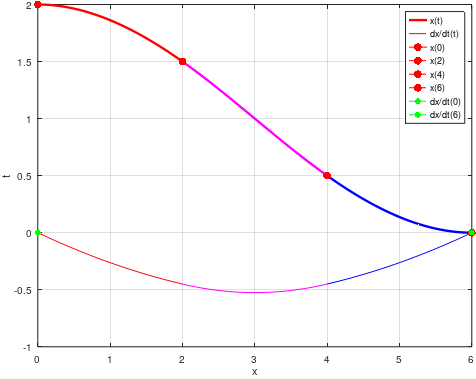
\includegraphics[width=1\textwidth, height=0.7\textwidth]{fig1}
            \caption{\label{fig:2a}}
        \end{subfigure}
        \begin{subfigure}{0.49\textwidth}
            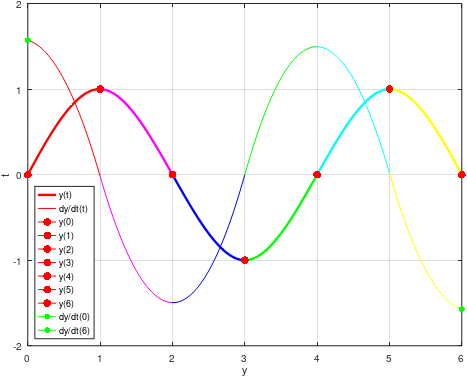
\includegraphics[width=1\textwidth, height=0.7\textwidth]{fig2}
            \caption{\label{fig:2b}}
        \end{subfigure}
        \caption{Gráficas de las componentes \(x\) (\subref{fig:2a}) e \(y\) (\subref{fig:2b}) con cada tramo diferenciado por color.}
        \label{fig1}
    \end{figure}

    \begin{figure}[h]
        \centering
        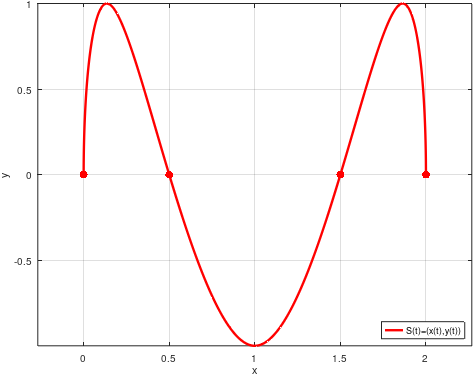
\includegraphics[width=0.5\textwidth]{fig3}
        \caption{Trayectoria seguida por la partícula.}
        \label{fig2}
    \end{figure}
    
    \section{Integración}
    Para calcular la distancia recorrida por la partícula en los \(6 segundos\) utilizaremos el método de fórmulas de Newton-Cotes y el método de Cuadraturas de Gauss con polinomios de Legendre.\\
    \indent El primero consiste en tomar \(n+1\) nodos \(x_i=x_0+ih\) para \(i=0,1,...,n\) donde \(x_0=a\), \(x_n=b\) y \(h=(b-a)/n\) equidistantes dentro del intervalo y construir un polinomio de Lagrange a partir de estos nodos, para luego aproximar la integral a partir de la integral de este polinomio en el intervalo.\\
    \indent El método de Cuadraturas de Gauss con Polinomios se basa en polinomios ortogonales, en este caso específico los de Legendre, los cuales están definidos en el dominio \([-1,1]\). El mismo encuentra tanto los puntos como los pesos para la evaluación en esos puntos que generen la mejor aproximación. Para los primero, utiliza las raíces de los polinomios ortogonales, y los pesos son determinados a partir de propiedades de los mismos.\\
    \indent Si dividimos el intervalo en L subintervalos y aplicamos estos métodos en cada uno de ellos, podemos obtener una mejor aproximación. Veremos cuántos subintervalos se requieren para lograr 6 dígitos exactos en la integral, empezando desde \(L=1\) intervalos y duplicando en cada iteración, hasta que la diferencia absoluta con la iteración anterior sea menor a \(1*10^{-7}\)\\\\\\\\
    \begin{figure}[h]
        \centering
        \begin{subfigure}{0.49\textwidth}
            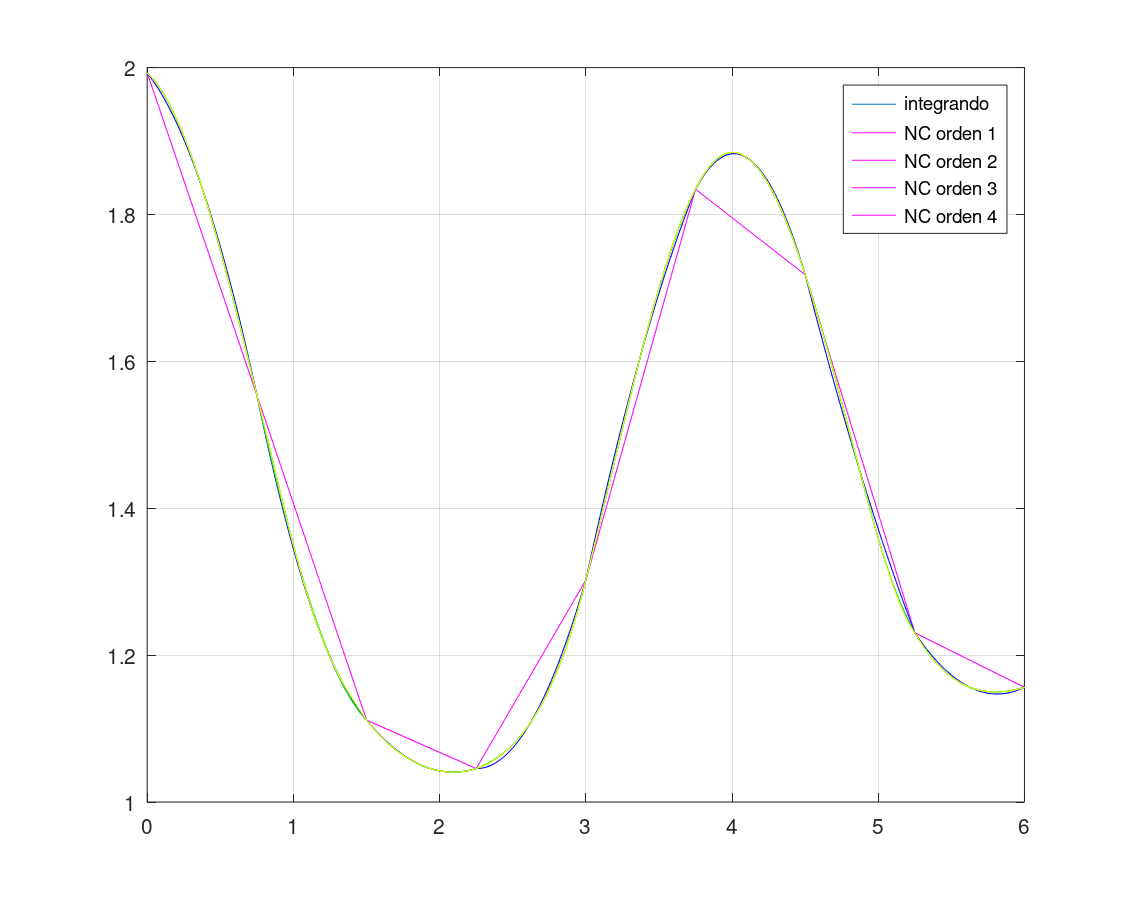
\includegraphics[width=1\textwidth, height=0.7\textwidth]{fig4}
            \caption{\label{fig:3a}}
        \end{subfigure}
        \begin{subfigure}{0.49\textwidth}
            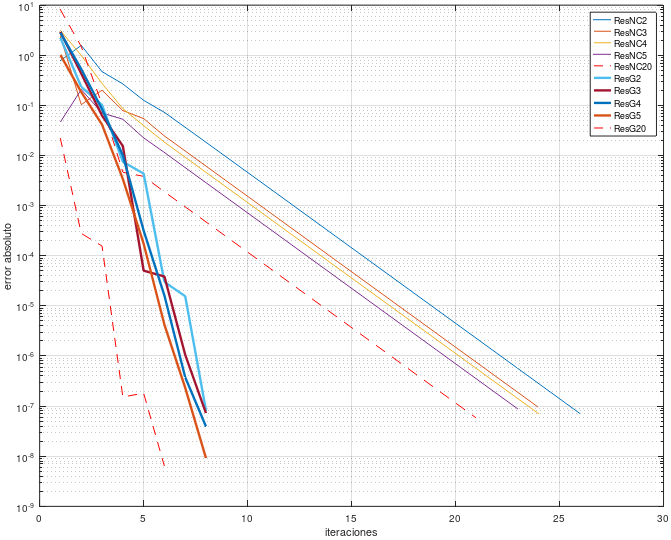
\includegraphics[width=1\textwidth, height=0.7\textwidth]{fig5}
            \caption{\label{fig:3b}}
        \end{subfigure}
        \captionsetup{justification=centering}
        \caption{Gráficas de los polinomios interpolantes de Newton-Cotes en 8 tramos (\subref{fig:3a}) y la curva del error desde \(L=2\) (\subref{fig:3b}).}
        \label{fig3}
    \end{figure}
    \indent A partir de estos métodos estimamos una distancia recorrida por la partícula de \(\int_{0}^{T} \sqrt{x_1'(t)^2+x_2'(t)^2}dt=\textbf{6.514997}\)
    \begin{table}[h]
        \centering
        \begin{tabular}{|l|l|l|}
            \hline
            \textbf{Método} & \textbf{tiempo{[}s{]}} & \textbf{L} \\ \hline
            NC n=2          & 124.7712018489838      & 67108864   \\ \hline
            NC n=3          & 43.19980502128601      & 16777216   \\ \hline
            NC n=4          & 57.75703001022339      & 16777216   \\ \hline
            NC n=5          & 35.19215083122253      & 8388608    \\ \hline
            NC n=20         & 36.19845604896545      & 2097152    \\ \hline
            Gauss-L n=2     & 0.6471190452575684     & 256        \\ \hline
            Gauss-L n=3     & 0.6503341197967529     & 256        \\ \hline
            Gauss-L n=4     & 0.6206791400909424     & 256        \\ \hline
            Gauss-L n=5     & 0.6107208728790283     & 256        \\ \hline
            Gauss-L n=20    & 0.1515882015228271     & 64         \\ \hline
        \end{tabular}
        \caption{Resultados de distintos métodos de integración numérica.}
        \label{Tabla}
    \end{table}
    \section{Conclusiones}
    Se comprobó a través de estos pasos que la interpolación por Splines Cúbicos genera no solo una curva considerablemente suave a partir de pocos datos de entrada, sino también que a partir de esta podemos aproximar el comportamiento de las componentes de la posición por separado, y que la curva que generarán ambas también será suave.\\
    \indent Además, vemos que por este método también obtenemos una expresión para las derivadas de las componente, a partir de las cuales podemos evaluar la velocidad instantánea de la partícula, además de usarla para estimar las distancia recorrida por la misma.\\
    \indent Respecto a la estimación de la distancia, la cual requiere el cálculo de una integral, observamos una diferencia considerable en el tiempo de cómputo requerido por cada método para llegar a la precisión requerida. En el caso de las fórmulas de Newton-Cotes, se logra una mejora considerable al aumentar el grado de los polinomios interpolantes, aunque al usar una cantidad mayor de nodos no necesariamente mejoraremos el método, debido a la cantidad de evaluaciones requeridas y a la naturaleza oscilante de los polinomios. En el caso de el método de Cuadratura de Gauss este parámetro no genera gran diferencia en el tiempo de cómputo, debido a que aumentan la cantidad de evaluaciones de la función.

    \section{Scripts Utilizados}
    \subsection{Script Cliente}
    \begin{lstlisting}[language=Octave]
    clc; clear all; close all;
    format long g;
    
    % - Mediciones
    tx = [0 2 4 6];         %tiempo de la medicion
    posx = [2.0 1.5 0.5 0.0]; %valor en x
    ty = [0 1 2 3 4 5 6];
    posy = [0.0 1.0 0.0 -1.0 0.0 1.0 0.0];
    
    a=0;
    b=6;
    
    dy0 = pi/2;
    dyn = -pi/2;
    
    % - a) Interpolacion
    [x,dx] = funcion_spline(tx,posx,0,0);   %velocidad inicial y final nulas en x
    [y,dy] = funcion_spline(ty,posy,pi/2,-pi/2);
    
    % - b) Grafica
      % x(t) y dx(t)
    figure(1);
    t = linspace(0,2,50);
    plot(t,x(t),'-r','linewidth',2);
    hold on;
    plot(t,dx(t),'-r');
    t = linspace(2,4,50);
    plot(t,x(t),'-m','linewidth',2);
    plot(t,dx(t),'-m');
    t = linspace(4,6,50);
    plot(t,x(t),'-b','linewidth',2);
    plot(t,dx(t),'-b');
    
    grid on;
    legend("x(t)","dx/dt(t)");
    xlabel("x");
    ylabel("t");
    
      % puntos (t,posx)
    for i=1:length(tx)
      plot(tx(i),posx(i), 'color', 'r', 'markersize', 20, 'displayname', strcat("x(", num2str(tx(i)),")"));
    endfor
    plot(0,0,'color','g','markersize',15,'displayname','dx/dt(0)');
    plot(6,0,'color','g','markersize',15,'displayname','dx/dt(6)');
    
    figure(2);
      % y(t) y dy(t)
    t = linspace(0.001,1,50);
    plot(t,y(t),'-r', 'linewidth',2);
    hold on;
    plot(t,dy(t),'-r');
    t = linspace(1,2,50);
    plot(t,y(t),'-m', 'linewidth',2);
    plot(t,dy(t),'-m');
    t = linspace(2,3,50);
    plot(t,y(t),'-b', 'linewidth',2);
    plot(t,dy(t),'-b');
    t = linspace(3,4,50);
    plot(t,y(t),'-g', 'linewidth',2);
    plot(t,dy(t),'-g');
    t = linspace(4,5,50);
    plot(t,y(t),'-c', 'linewidth',2);
    plot(t,dy(t),'-c');
    t = linspace(5,6,50);
    plot(t,y(t),'-y', 'linewidth',2);
    plot(t,dy(t),'-y');
    
    grid on;
    h = legend("y(t)","dy/dt(t)");
    legend(h,"location","southwest");
    xlabel("y");
    ylabel("t");
    
      % puntos (t,posy)
    for i=1:length(ty)
      plot(ty(i),posy(i), 'color', 'r', 'markersize', 20, 'displayname', strcat("y(", num2str(ty(i)),")"));
    endfor
    plot(0,dy0,'color','g','markersize',15,'displayname','dy/dt(0)');
    plot(6,dyn,'color','g','markersize',15,'displayname','dy/dt(6)');
    
      % (x(t),y(t))
    figure(3);
    h=ezplot(x,y,[0 6]);
    set(h,'color','r','linewidth',2);
    hold on;
      % puntos (posx,posy)
    for i=1:length(tx)
      plot(x(tx(i)),y(tx(i)), 'color', 'r', 'markersize', 20, 'displayname', strcat("S(", num2str(tx(i)),")"));
    endfor
    
    grid on;
    h=legend("S(t)=(x(t),y(t))");
    legend(h,"location","southeast");
    
    % b) Evaluacion
    % S(3)
    pos3 = [x(3),y(3)]
    % dS(3)
    vel3 = [dx(3),dy(3)]
    
    % c) Integración
    integrando = @(t) sqrt(dx(t).^2 + dy(t).^2);
    
      % Grafica del integrando con los polinomios interpolantes por subintervalo
    figure(4);
    t = linspace(0.0001,6,100);
    plot(t,integrando(t),'linewidth',2);
    hold on;
    
    h = (b-a)/8;
        % n=2 (Trapecio)
    for i=1:8
      p = linspace(a+(i-1)*h,a+i*h,2);
      fp = integrando(p);
      P = PolyLag(p,fp);
      t = linspace(a+(i-1)*h,a+i*h,50);
      plot(t,polyval(P,t),'-m');
    endfor
        % n=3 (Simpson)
    for i=1:8
      p = linspace(a+(i-1)*h,a+i*h,3);
      fp = integrando(p);
      P = PolyLag(p,fp);
      t = linspace(a+(i-1)*h,a+i*h,50);
      plot(t,polyval(P,t),'-b');
    endfor
        % n=4
    for i=1:8
      p = linspace(a+(i-1)*h,a+i*h,4);
      fp = integrando(p);
      P = PolyLag(p,fp);
      t = linspace(a+(i-1)*h,a+i*h,50);
      plot(t,polyval(P,t),'-g');
    endfor
        % n=5
    for i=1:8
      p = linspace(a+(i-1)*h,a+i*h,5);
      fp = integrando(p);
      P = PolyLag(p,fp);
      t = linspace(a+(i-1)*h,a+i*h,50);
      plot(t,polyval(P,t),'-y');
    endfor
    legend('integrando','NC orden 1','NC orden 2','NC orden 3','NC orden 4');
    
    % Calculo de la integral
    tolerancia = 1e-7;
    maxit = 30;
    
    [INC2,itNC2,rNC2,tNC2,LNC2] = intNC(integrando,0,6,2,tolerancia,maxit);
    INC2
    itNC2
    tNC2
    LNC2
    
    [INC3,itNC3,rNC3,tNC3,LNC3] = intNC(integrando,0,6,3,tolerancia,maxit);
    INC3
    itNC3
    tNC3
    LNC3
    
    [INC4,itNC4,rNC4,tNC4,LNC4] = intNC(integrando,0,6,4,tolerancia,maxit);
    INC4
    itNC4
    tNC4
    LNC4
    
    [INC5,itNC5,rNC5,tNC5,LNC5] = intNC(integrando,0,6,5,tolerancia,maxit);
    INC5
    itNC5
    tNC5
    LNC5
    
    [INC20,itNC20,rNC20,tNC20,LNC20] = intNC(integrando,0,6,20,tolerancia,maxit);
    INC20
    itNC20
    tNC20
    LNC20
    disp("===================================");
    
    [IG2,itG2,rG2,tG2,LG2] = intGauss(integrando,0,6,2,tolerancia,maxit);
    IG2
    itG2
    tG2
    LG2
    
    [IG3,itG3,rG3,tG3,LG3] = intGauss(integrando,0,6,3,tolerancia,maxit);
    IG3
    itG3
    tG3
    LG3
    
    [IG4,itG4,rG4,tG4,LG4] = intGauss(integrando,0,6,4,tolerancia,maxit);
    IG4
    itG4
    tG4
    LG4
    
    [IG5,itG5,rG5,tG5,LG5] = intGauss(integrando,0,6,5,tolerancia,maxit);
    IG5
    itG5
    tG5
    LG5
    
    [IG20,itG20,rG20,tG20,LG20] = intGauss(integrando,0,6,20,tolerancia,maxit);
    IG20
    itG20
    tG20
    LG20
    
    % Graficar residuos
    figure(5);
    semilogy(rNC2);
    hold on;
    semilogy(rNC3);
    semilogy(rNC4);
    semilogy(rNC5);
    semilogy(rNC20,'color','r','linestyle','--');
    semilogy(rG2,'linewidth',2);
    semilogy(rG3,'linewidth',2);
    semilogy(rG4,'linewidth',2);
    semilogy(rG5,'linewidth',2);
    semilogy(rG20,'color','r','linestyle','--');
    legend('ResNC2', 'ResNC3', 'ResNC4', 'ResNC5', 'ResNC20', 'ResG2', 'ResG3', 'ResG4', 'ResG5', 'ResG20');
    xlabel('iteraciones');
    ylabel('error absoluto');
    \end{lstlisting}
    \subsection{cubic\_spline\_clamped}
    \begin{lstlisting}[language=Octave]
    % x: puntos xi, i=1,2,...,n
    % y: puntos yi correspondiente a f(xi), i=1,2,...,n
    % df1 y dfn: valor de la derivada de f en x0 y xn
    function [ai,bi,ci,di] = cubic_spline_clamped(x,y,df1,dfn)
        n = length(x);
    
        ai = y;
    
        h(1:n-1) = x(2:n) - x(1:n-1);
    
        % - Calculamos los terminos independientes
        b(1:n) = 0;
        b(1) = 3*( (y(2) - y(1))/h(1) - df1 );    %fila 1
        b(2:n-1) = 3*( (y(3:n) - y(2:n-1))./h(2:n-1) - (y(2:n-1) - y(1:n-2))./h(1:n-2) );   %filas 2...n-1
        b(n) = 3*( dfn - (y(n) - y(n-1))/h(n-1) );    %fila n
    
        % - Calculamos (metodo de crout)
        l(1) = 2*h(1); 
        u(1) = 0.5;
        z(1) = b(1)/l(1);
    
        for i = 2:n-1
            l(i) = 2 * ( x(i+1)-x(i-1) ) - h(i-1) * u(i-1);
            u(i) = h(i) / l(i);
            z(i) = (b(i) - h(i-1) * z(i-1) ) / l(i);
        endfor
    
        l(n) = h(n-1) * (2-u(n-1));
        z(n) = (b(n) - h(n-1)*z(n-1) ) / l(n);
        ci(n) = z(n);
    
        % Paso 7:
        for i = n-1:-1:1
            ci(i) = z(i) - u(i) * ci(i+1);
            bi(i) = (y(i+1)-y(i))/ h(i) - h(i) * ( ci(i+1) + 2 * ci(i) ) / 3;
            di(i) = (ci(i+1)-ci(i))/(3*h(i));
        endfor
    
        ai = y(1:n-1)';
        bi = bi';
        ci = ci(1:n-1)';
        di = di';
    endfunction
    \end{lstlisting}
    
    \subsection{funcion\_spline}
    \begin{lstlisting}[language=Octave]
    function [S,dS]=funcion_spline(x1,y1,df1=0,df2=0)
        % extremos sujetos
        [a,b,c,d] = cubic_spline_clamped(x1,y1,df1,df2);
        % extremos libres
        %[a,b,c,d] = cubic_spline_natural(x1,y1);
    
        S=@(x) a(1)*(x==x1(1));
    
        M=[d c b a];
        dM=[];
        dS= @(x) 0;
        for i=1:length(x1)-1
            dM=[dM;polyder(M(i,:))];
            S=@(x) S(x) + polyval(M(i,:),x-x1(i)).*(x>x1(i)).*(x<=x1(i+1));
            dS=@(x) dS(x) + polyval(dM(i,:),x-x1(i)).*(x>x1(i)).*(x<=x1(i+1));
        endfor
    endfunction
    \end{lstlisting}
    
    \subsection{gauss\_xw}
    \begin{lstlisting}[language=Octave]
    function [x, w] = gauss_xw(n)
        % [x, w] = gauss_xw(n)
        % Genera las abscisas y pesos para la Cuadratura Gauss-Legendre.
        % n: numero de puntos de integracion
        % x: abscisas de la cuadratura
        % w: pesos de la cuadratura
        x = zeros(n,1);
        w = x;
        m = (n+1)/2;
        for ii=1:m
            z = cos(pi*(ii-.25)/(n+.5)); % estimado Inicial.
            z1 = z+1;
            while abs(z-z1)>eps
                p1 = 1;
                p2 = 0;
                for jj = 1:n
                    p3 = p2;
                    p2 = p1;
                    p1 = ((2*jj-1)*z*p2-(jj-1)*p3)/jj; % El polinomial. Legendre
                endfor
                pp = n*(z*p1-p2)/(z^2-1); % La L.P. Derivada.
                z1 = z;
                z = z1-p1/pp;
            endwhile
            x(ii) = -z; % Construye las abscissas.
            x(n+1-ii) = z;
            w(ii) = 2/((1-z^2)*(pp^2)); % Construye los pesos.
            w(n+1-ii) = w(ii);
        endfor
    endfunction
    \end{lstlisting}
    
    \subsection{intGauss}
    \begin{lstlisting}[language=Octave]
    function [I,it,r,t,L] = intGauss(f,a,b,n,tolerancia,maxit)
      % aproxima la integral de f sobre [a,b],
      %subdividiendo en L subintervalos
    
      tic();
    
      % calculamos los pesos y los puntos a evaluar t una sola vez
      [xg,w] = gauss_xw(n);
      t = linspace(-1,1,n);
    
      L=1;
      h=b-a;
    
      y=linspace(a,b,L+1);
      I=0;
      for i=1:L
        t = h/2*(xg+1)+y(i);
        I += h/2*(w'*f(t));
      endfor
      % -------------
      for it=2:maxit
        % duplicamos los subintervalos
        L=L*2;
        h=h/2;
    
        y=linspace(a,b,L+1);
        I1=0;
        for i=1:L
          t = h/2*(xg+1)+y(i);
          I1 += h/2*(w'*f(t));
        endfor
    
        %residuo
        r(it-1) = abs(I1-I);
        if r(it-1) < tolerancia
          I = I1;
          break;
        endif
    
        I = I1;
      endfor
    
      t = toc();
    
      if it == maxit
        disp("la integral no converge para maxit iteraciones");
      endif
    endfunction
    \end{lstlisting}
    
    \subsection{intNC}
    \begin{lstlisting}[language=Octave]
    function [I,it,r,t,L] = intNC(f,a,b,n,tolerancia,maxit)
      % aproxima la integral de f sobre [a,b]
      % utilizando la formula de Newton-Cotes compuesta
      % de n puntos, subdividiendo en L subintervalos
    
      tic();
    
      % calculamos los pesos una sola vez
      w = pesosNC(n);
    
      L=1;
      h = b-a;
      y = linspace(a,b,L+1);
      % crea una matriz con los puntos a evaluar
      x = linspace(0, 1, n).' * (y(2:end) - y(1:end-1)) + y(1:end-1);
      x = reshape(x, [], L);
    
      fx = f(x);
      I = sum(h * (fx .* w)(:));
      % -------------
      for it=2:maxit
        % duplicamos los subintervalos
        L=L*2;
        h = h/2;
        y = linspace(a,b,L+1);
        % crea una matriz con los puntos a evaluar
        x = linspace(0, 1, n).' * (y(2:end) - y(1:end-1)) + y(1:end-1);
        x = reshape(x, [], L);
    
        fx = f(x);
        I1 = sum(h * (fx .* w)(:));
    
        %residuo
        r(it-1) = abs(I1-I);
        if r(it-1) < tolerancia
          I = I1;
          break;
        endif
    
        I = I1;
      endfor
    
      t = toc();
    
      if it == maxit
        disp("la integral no converge para maxit iteraciones");
      endif
    endfunction
    \end{lstlisting}
    
    \subsection{pesosNC}
    \begin{lstlisting}[language=Octave]
    function w = pesosNC(n)
        % function w = pesosNC(n)
        % se calculan los pesos
        % de la formula de Newton-Cotes de n puntos
        x = linspace(0,1,n);
        A = ones(n,n);
        for i=2:n
          A(i,:) = A(i-1,:) .* x;
        end
        b = 1./(1:n)';
        w = A\b;
    endfunction
    \end{lstlisting}
    
    \subsection{PolyLag}
    \begin{lstlisting}[language=Octave]
    %P: vector de coeficientes del polinomio de Lagrange que interpola los puntos (x,y)
    %x: valores que toman los puntos interpolantes
    %y: valores de la funcion interpolada en los puntos x[i]
    function [P] = PolyLag (x,y)
      n = length(x);
    
      % calculamos el primer miembro solo para no enquilombarnos de indices despues
      L1 = [1 (-1)*x(2)];               %(x - x_2)
      div = x(1)-x(2);                  %(x_1 - x_2)
      for i=3:n
        L1 = conv(L1, [1 (-1)*x(i)]);   %(x - x_2)(x - x_3)(x - x_4)...(x - x_n)
        div = div*(x(1)-x(i));          %(x_1 - x_2)(x_1 - x_3)(x_1 - x_4)...(x_1 - x_n)
      endfor
      P = L1 * (y(1)/div);              %f(x_1)*(x - x_2)(x - x_3)(x - x_4)...(x - x_n) / (x_1 - x_2)(x_1 - x_3)(x_1 - x_4)...(x_1 - x_n)
    
      % calculamos el resto de miembros del polinomio
      for i=2:n
        % inicializamos el i-esimo miembro del polinomio de Lagrange
        % es lo mismo que para el primero
        Laux = [1 (-1)*x(1)];
        div = x(i)-x(1);
    
        for j=2:n
          if j!=i                       %evitamos (x - x_i) y (x_i - x_i)
            Laux = conv(Laux, [1 (-1)*x(j)]);
            div = div*(x(i)-x(j));
          endif
        endfor
        P = P + Laux * (y(i)/div);
      endfor
    
    endfunction
    \end{lstlisting}
\end{document}
